\documentclass[11pt,a4paper]{article}

\bibliographystyle{ieeetr}

\usepackage[margin=1in]{geometry}
\usepackage{graphicx}
\usepackage{subfig}
\usepackage{amsmath}
\usepackage{url}
\usepackage{diagbox}
\usepackage{enumitem}
\usepackage{braket}

\usepackage{tikz}
\usetikzlibrary{chains} % TM tape
\usetikzlibrary{automata,positioning}   % automaton diagram

\newenvironment{turing}[2]{
    \begin{enumerate}[leftmargin=0pt,labelsep=0pt,align=left,parsep=0pt]
        \item[$#1={}$]``\ignorespaces#2
            \begin{enumerate}[
                nosep,
                align=left,
                labelwidth=1.5em,
                label=\bfseries\arabic{*}.,
                ref=\arabic{*}
            ]}{\unskip''
            \end{enumerate}
    \end{enumerate}}

\newcommand{\bitem}{\item\hspace*{1em}\ignorespaces}

\title{Cellular Automata and Computational Universality}

\begin{document}

\maketitle

\begin{center}
    Thomas Archbold \\
    University of Warwick \\
    \texttt{T.Archbold@warwick.ac.uk}
\end{center}

\begin{abstract}
    Cellular automata are discrete models with the ability to not only give rise
    to beautiful, intricate patterns, but also to be used as powerful tools of
    computation, with applications in cryptography, error-correction coding, and
    simulation of computer processors, to name a few. They also raise profound
    questions about the nature of our reality, asking whether our universe could
    be one such automaton. This paper provides a discussion into these automata,
    exploring the various power and limitations of a number of specific rule
    sets, covering John Conway's well-known ``Game of Life'' to the more obscure
    ``Langton's ant'' and ``Wireworld''. In particular, it explores the notion
    of computational universality, or Turing completeness, an automaton's
    ability to simulate any conceivable computation, and considers their
    potential in the context of solving two specific problems, the Firing Squad
    Synchronisation Problem and the Majority Problem. Existing solutions to
    these problems are explored, and their existing avenues for optimisation are
    discussed. In order to fully appreciate the complex structures that can
    arise from such simple beginnings, this project also presents software to
    visualise and probe further into the nature of the automata highlighted.
\end{abstract}

\section{Introduction}
    A cellular automaton is a discrete model of computation which consists of a
    finite collection of ``cells'', each in one of a finite number of states.
    The state of each of these cells may evolve over the progression of time in
    discrete steps, and may do so according to a deterministic set of rules
    based on the states of neighbouring cells. Their inherently discrete nature
    allows for strong analogies to be made with digital computers, and gifts
    them the ability to simulate digital processes and the potential to solve
    problems in this area.
    
    Consider the cellular automaton defined by the simple rule:
    \begin{equation}
        \label{eq:rule90}
        a_{i}^{t+1} = a_{i-1}^{t} + a_{i+1}^{t} \mod{2}
    \end{equation}

    For any automaton, in each time step the rule is applied to all cells in the
    automaton instantaneously and simultaneously. In this case, our set of
    states is ${0,1}$, and for each cell we look at the cells immediately
    preceding and succeeding it: if exactly one of them is in state 1, then this
    cell will be in state 1 in the next time step. Otherwise it will be in state
    0.

    \begin{figure}[h]
        \begin{center}
            \includegraphics[width=4in]{rule90.png}
            \caption{Pattern generated from applying Eq. 1 over 129 generations}
            \label{fig:rule90}
        \end{center}
    \end{figure}

    \subsection{Self-similarity}
    Figure \ref{fig:rule90} shows a visualisation of Eq. \ref{eq:rule90}. A cell is
    filled white if it has the value 1, and black otherwise. Note that each new
    ``line'' of the visualisation represents the automaton in the next
    successive time-step from the one before; this automaton is one-dimensional,
    and so we may represent it in its entirety as a single row of cells. This
    pattern exhibits two important characteristics, the first of which is
    ``self-similarity'', meaning that portions of the pattern generated are
    indistinguishable from the whole when magnified. As Wolfram states, in this
    way ``the pattern is therefore invariant under rescaling... and may be
    characterised by a fractal dimension'' \cite{WolframFractal}. One such
    definition of this is the Hausdorff-Besicovitch dimension \cite{Hausdorff}.

    As an example, suppose we have a cube with some mass, and we wish to find
    out how the mass scales when we try to make the same cube out of smaller
    copies of the original. Intuitively, one way to do this require eight
    smaller cubes, each of whose side length is half that of the original cube.
    So with the scaling factor of $\frac{1}{2}$, the mass of each smaller cube
    is $\frac{1}{8} = (\frac{1}{2})^3$.
    So we arrive at the equation $N = S^D$, where $N$ is the number of smaller
    copies that can be stuck together to make the original, $S$ is the scaling
    factor of these smaller copies, and $D$ is the dimension. In this example, we
    compute that the dimension of a cube is 3, which is obviously correct.  Back
    to the dimension of the Sierpinski Triangle, we can see that each larger
    triangle is made up of three smaller triangles, each of whose side lengths
    are half that of the larger triangle. So we calculate the dimension as:

    \begin{equation}
        \label{sierpinskiDim}
        \begin{split}
            \tfrac{1}{3} &= (\tfrac{1}{2})^D \\
            \log{\tfrac{1}{3}} &= D \log{\tfrac{1}{2}} \\
            D &= \tfrac{\log{3}}{\log{2}} \approx 1.585
        \end{split}
    \end{equation}

    Many naturally-occurring systems exhibit fractal structures, from snowflakes
    to pine cones to Romanesco broccoli, and raises the possibility that these
    are generated through the evolution of some natural cellular automata or
    similar processes.

    \begin{figure}[h]%
        \centering
        \subfloat[Snowflake]{{\includegraphics[width=5cm]{snowflake.jpg}}}%
        \qquad
        \subfloat[Romanesco broccoli]{{\includegraphics[width=5cm]{romanesco_broccoli.jpg}}}%
        \caption{Snowflakes and Romanesco broccoli exhibit fractal structures}%
        \label{fig:nature_fractals}%
    \end{figure}

    \subsection{Self-organisation}
    Second of the characteristics exhibited by this cellular automaton is
    ``self-organisation'', whereby from an initial disorderly or chaotic state
    there appear ordered structures seemingly spontaneously. This is illustrated
    in Fig. \ref{fig:self-organisation} below: one can clearly see the emergence
    of similar triangular structures in the cone snail's shell, appearing from a
    chaotic background. This starting chaos is modelled in the cellular
    automaton by randomly assigning each cell a value of 0 or 1, with each
    occurring with probability one half.

    \begin{figure}[h]%
        \centering
        \subfloat[Shell of a cone
        snail]{{\includegraphics[width=2in]{cone_shell.jpg}}}%
        \qquad
        \subfloat[Rule 90 with random starting
        configuration]{{\includegraphics[width=2in]{rule90_rand.png}}}%
        \caption{Natural processes can exhibit structures found in automata}
        \label{fig:self-organisation}
    \end{figure}

\section{Classifying automata}
    In order to classify automata, we can take into account both the size of the
    neighbourhood each cell considers going into the next generation, as well as
    the number of possible states in which a cell may be. Call these $N$ and $Q$
    respectively; in the case of Eq. \ref{eq:rule90}, $N=3$ and $Q=2$, and so the
    total number of different ``transitions'' from one state to the next is $N^Q
    = 8$. We may write out all of these transitions as follows:

    \begin{table}[h]
        \centering
        \begin{tabular}{c|c|c|c|c|c|c|c}
            111 & 110 & 101 & 100 & 011 & 010 & 001 & 000 \\
            \hline
            0   & 1   & 0   & 1   & 1   & 0   & 1   & 0
        \end{tabular}
    \end{table}

    Reading the bottom row of this transition table, we get the binary number
    $01011010_{\text{bin}} = 90_{\text{dec}}$, and so we name this rule set Rule
    90. Using this convention, we may now construct our own automata based
    solely on the knowledge of its name (at least for elementary cellular
    automata). For example, take Rule 110, introduced by Wolfram 1983
    \cite{WolframRule110}. We first convert $110_{\text{dec}}$ to binary, and
    then use this to fill in the table as above:

    \begin{table}[h]
        \begin{minipage}{.5\linewidth}
            \centering
            \begin{tabular}{c|c|c|c|c|c|c|c}
                111 & 110 & 101 & 100 & 011 & 010 & 001 & 000 \\
                \hline
                ? & ? & ? & ? & ? & ? & ? & ?
            \end{tabular}
        \end{minipage}%
        $ \Rightarrow $
        \begin{minipage}{.6\linewidth}
            \begin{tabular}{c|c|c|c|c|c|c|c}
                111 & 110 & 101 & 100 & 011 & 010 & 001 & 000 \\
                \hline
                0 & 1 & 1 & 0 & 1 & 1 & 1 & 0
            \end{tabular}
        \end{minipage}
    \end{table}

    To convert this to a concrete set of rules to simulate in a computer
    programs (in a more elegant way than a collection of eight \texttt{if}
    statements), we can put the information we have gathered so far in a
    Karnaugh map to get a Boolean algebraic expression of the ruleset, as in the
    table below. We use $A$ , $B$, and $C$ to denote $a_{i-1}$, $a_i$, and
    $a_{i+1}$, at time $t$, respectively. From this we can reduce the ruleset to
    the Boolean expression in Eq. \ref{eq:rule110} by observation.

    \begin{table}[h]
        %\caption{The Karnaugh map resulting from decoding Rule 110}
        %\label{kmap}
        \centering
        \begin{tabular}{|c||c|c|c|c|}\hline
            \diagbox{C}{AB} & 00 & 01 & 11 & 10 \\
            \hline
            0 & 0  & 1  & 1  & 0    \\
            \hline
            1 & 1  & 1  & 0  & 1    \\
            \hline
        \end{tabular}
    \end{table}

    \begin{equation}
        \label{eq:rule110}
        \begin{split}
            B^{t+1} &= \overline{A} \cdot C + B \cdot \overline{C} + \overline{B} \cdot C \\
            &= \overline{A} \cdot C + B \oplus C
        \end{split}
    \end{equation}

    The resulting visualisation in Fig. \ref{fig:rule110} exhibits similar
    characteristic of self-organisation, however it is hard to say whether it
    shows self-similarity as well.

    \begin{figure}[h]
        \begin{center}
            \includegraphics[width=4in]{rule110.png}
            \caption{Rule 110 generated using Eq. \ref{eq:rule110}}
            \label{fig:rule110}
        \end{center}
    \end{figure}

    \subsection{Elementary cellular automata}
    Elementary cellular automata are the simplest class of one-dimensional
    cellular automata; each cell may be in one of two states, 0 or 1, and rule
    sets only take into account the cell itself and its immediate neighbours
    (the nearest cell left and right of the cell being computed). Since there
    are a total of $2^3=8$ combinations of values for a neighbourhood of cells,
    and each of these neighbourhoods causes a cell to move to one of two states
    in the next generation, this means there are $2^8=256$ elementary cellular
    automata. Their evolution is often illustrated by each progressive ``new
    line'' showing the next generation of the automaton, as caused by applying
    the rule set to the current generation.
    
    Two technically different automata may give rise to similar patterns, and
    indeed many automata are equivalent to each other thanks to simple
    transformations of their underlying geometry. The first of these
    transformations is reflection in the vertical axis; the result of applying
    this is known as the mirror rule \cite{elementary}. For example, take Rule
    30. Each time some neighbourhood produces a live cell in Rule 30, let's take
    this neighbourhood and reflect it in the vertical plane, giving the table
    below:

    \begin{table}[h]
        \centering
        \begin{tabular}{|c|c|c|c|c|c|c|c|}\hline
            111 & 110 & 101 & 100 & 011 & 010 & 001 & 000   \\
            \hline
            0 & 0 & 0 & 1 & 1 & 1 & 1 & 0   \\
            \hline
            0 & 1 & 0 & 1 & 0 & 1 & 1 & 0   \\
            \hline
        \end{tabular}
    \end{table}

    The first line of the table shows the ruleset for Rule 30, while the line
    below gives that of our new ruleset, made by applying the mirror rule to
    Rule 30. Thus we get Rule 30's mirror rule, Rule $01010110_{\text{bin}}$ =
    Rule $86_{\text{dec}}$. Rules which generate the same ruleset under
    mirroring are called amphichiral, and of the 256 elementary cellular
    automata, 64 are so.

    The second of these transformations is to exchange the roles of 0s and 1s in
    the ruleset definition, and doing so is applying the complement rule
    \cite{elementary}.  Again applying this to Rule 30, we get the table below
    (note that the roles of 0s and 1s are exchanged in both the top and bottom
    rows):

    \begin{table}[h]
        \centering
        \begin{tabular}{|c|c|c|c|c|c|c|c|}\hline
            000 & 001 & 010 & 011 & 100 & 101 & 110 & 111   \\
            \hline
            1 & 1 & 1 & 0 & 0 & 0 & 0 & 1   \\
            \hline
        \end{tabular}
    \end{table}

    So we arrive at Rule $10000111_{\text{bin}} = 135_{\text{dec}}$ as the
    complement of Rule 30. There are 16 rules which are the same as their
    complement.
    Both of these rules can be applied at once to a ruleset, and the result is
    Rule 149 when applied to Rule 30. There are 16 rules which are the same as
    their mirrored complementary rules. There are 88 rules which are
    inequivalent under these transformations \cite{elementary}.

    \subsection{Wolfram classes}
    Wolfram gives the following classes for categorising the behaviours of
    different automata:

    \begin{itemize}
        \item Class One: rapidly converge to a uniform state e.g. Rule 0, 232
        \item Class Two: rapidly converge to a stable or oscillating state e.g.
            Rule 250
        \item Class Three: appear to evolve in a chaotic fashion e.g. Rule 30,
            150, 182
        \item Class Four: form areas of repetitive or stable states, but also
            structures which interact in complicated ways e.g. Rule 54
    \end{itemize}

    Two of these 256 rules are particularly special, namely Rule 54 and 110,
    both of which are Class 4 elementary cellular automata. Rule 110 has been
    proven to be universal, or Turing complete, meaning it is theorectically
    able to simulate any function. Meanwhile, it is so far unknown whether Rule
    54 is capable of universal computation -- interacting structures form, but
    it remains to been seen whether structures useful for computation arise.
    Computational universality is discussed more in-depth later on.

    There have been attempts to classify automata more rigorously, and Culik and
    Yu proposed four well-defined classes for such a task; membership in such
    classes has, however, been shown to be undecidable \cite{CulikYuMembership}.

    \subsection{Two dimensional cellular automata}
    Two dimensional cellular automata become a bit more interesting than their
    dimensionally-deficient brethren. Rather than having a single row of cells
    to consider at each generation, now a two-dimensional plane of cells is used
    to compute the evolution of the automaton. Whereas elementary automata
    looked only at the neighbourhood of $a_{i-1}, a_i,$ and $a_{i+1}$ when
    applying the set of rules, two-dimensional automata typically have a larger
    neighbourhood to consider. Two of the most common types of neighbourhood are
    the Moore neighbourhood and the von Neumann neighbourhood
    \cite{neighbourhoods}. The former includes the 8 cells directly surrounding
    the current cell being considered, while the latter only focuses on the four
    orthogonally ajacent cells. Occasionally, one may use the extended von
    Neumann neighbourhood, for which the next four closest orthogonally adjacent
    cells are also included.

    Using a Moore neighbourhood and a set of states of size $k$, we can see that
    the total number of configurations for one particular neighbourhood is
    $k^9$, as each of the nine cells included in the neighbourhood may be in one
    of $k$ states. For an automaton such as Conway's Game of Life, where each
    cell is either alive or dead and a moore neighbourhood is used, there are
    $2^9=512$ ways to configure one of these neighbourhoods alone. The general
    equation for the number of automata for a given neighbourhood and number of
    possible states is $k^{k^n}$, where $k$ is the number of possible states and
    $n$ is the size of the neighbourhood used when determining the automaton's
    evolution between time steps (including the cell being computed); in the
    case of a two-dimensional automaton using two states and a Moore
    neighbourhood (such as Game of Life), there are $2^{2^9}$ possible automata
    \cite{num_rules}.

    \subsection{Game of Life and Life-like automata}
    At this point it makes sense to talk a bit more about Conway's Game of Life.
    It was invented in 1970 by the British mathematician John Conway, after
    developing an interest in them after their introduction by John von Neumann
    in the late 1940s, who aimed to discover a hypothetical machine that was
    capable of recreating itself \cite{GameOfLife}. Von Neumann was able to
    achieve this goal using a complex automaton, with 29 states and complicated
    rules to do so \cite{VonNeumannCA}. Von Neumann's automaton is discussed in
    more depth later. The Game of Life was thus Conway's way of simplifying von
    Neumann's ideas; in fact, not only can the Game of Life simulate the Game of
    Life, it is also capable of universal computation, a topic discussed more
    in-depth later. The rules for Game of Life are as follows:

    \begin{itemize}
        \item If the current cell $a_{i,j}^t$ is dead, then:
            \begin{itemize}
                \item if the number of alive surrounding cells is 2 or 3,
                    then $a_{i,j}$ will become alive in the next generation
                \item else $a_{i,j}$ remains dead
            \end{itemize}
        \item If the current cell $a_{i,j}^t$ is alive, then:
            \begin{itemize}
                \item if the number of alive surrounding cells is less than 2,
                    then $a_{i,j}$ dies as if through isolation
                \item if the number of alive surrounding cells is greater than
                    3, then $a_{i,j}$ dies as if through overcrowding
                \item else $a_{i,j}$ lives on to the next generation
            \end{itemize}
    \end{itemize}

    There are many fascinating structures which arise out of these simple rules,
    and can be classed as follows:

    \begin{itemize}
        \item Still Life - patterns that do not change at all from one
            generation to the next
        \item Oscillators - patterns which generate some sort of cycle of
            patterns in a fixed place with a specific period
        \item Gliders and Spaceships - patterns which cycle through some finite
            set of patterns, but whose position is shifted each time, appeaing
            to move
        \item Guns - repeating patterns which produce a spaceship after a finite
            number of generations
        \item Puffers - moving patterns which leave a trail of stable or
            oscillating debris at regular intervals
        \item Rakes - moving patterns which emit spaceships at regular intervals
            as they move
        \item Breeders - oscillating patterns which deposit guns at regular
            intervals. Unline guns, puffers, and rakes, who each have a linear
            growth rate, breeders exhibit exponential growth rate
    \end{itemize}

    On 6\textsuperscript{th} March, 2018 the first knightship was discovered by
    Adam P. Goucher, named Sir Robin \cite{Knightship}. A knightship is a
    spaceship which moves two squares horizontally for every square it moves
    vertically, as opposed to regular spaceships, which move only vertically or
    horizontally, or gliders, which move exactly diagonally. Sir Robin became
    the first new spaceship movement pattern for an elementary spaceship to be
    discovered in forty eight years \cite{fortyeight}.

    Conway originally believed that no pattern could grow infinitely, i.e. for
    the population to grow past any upper limit for some initial configuration
    with finite number of alive cells, and offered fifty dollars to the first
    person who could prove or disprove this conjecture before the end of 1970.
    In November of that year a team from the Massachusetts Institute of
    Technology, led by Bill Gosper, found a structure which produced gliders
    every 30 generations, and called it the Gosper Glider Gun. Later on, smaller
    patterns were found to produce infinite growth, one of which has been proven
    to be minimal, starting off with only ten alive cells
    \cite{infiniteGrowth}. More of what this means for the computational power
    of Game of Life, as well as other automata, will be discussed under
    Computational Universality.

    A cellular automaton is Life-like (similar to Game of Life) if it meets the
    following criteria \cite{LifeLike}:

    \begin{itemize}
        \item it is two-dimensional
        \item each cell of the automaton may be in one of two states, alive or
            dead (or on or off) at any point
        \item a cell's Moore neighbourhood is used to compute the cell's state
            in the next generation
        \item in each time step of the automaton, the next state of the cell can
            be expressed as a funciton of the number of adjacent cells that are
            in the alive state and of the cell's own state
    \end{itemize}

    As with elementary cellular automata, it is helpful to refer to specific
    rulesets in a more generalised way. Where this was using the rule's binary
    encoding for one-dimensional automata, one such convention for
    two-dimensional automat is using a string $Bx/Sy$, where $x$ and $y$ are a
    sequence of digits, 0 to 8, in ascending order. The presence of a digit $d$
    in $x$ means that a dead cell with $d$ alive neighbours will become alive in
    the next generation, while the presence of $d$ in $y$ signifies that an
    alive cell with $d$ alive neighbours will continue to live on to the next
    generation. For example, Game of Life is denoted B3/S23: a dead cell is
    \textbf{B}orn if there are exactly 3 alive neighbours surrounding it, and
    and alive cell \textbf{S}urvives if there are two or three alive cells
    surrounding it.

    \begin{figure}[h]
        \begin{centering}
            \begin{tabular}{cc}
                \includegraphics[width=2in]{replicator1.png} &
                \includegraphics[width=2in]{replicator2.png} \\
                \includegraphics[width=2in]{replicator3.png} &
                \includegraphics[width=2in]{replicator4.png} \\
            \end{tabular}
            \caption{Replicator (B1357/S1357) replicating itself over the course of
            56 generations}
        \end{centering}
    \end{figure}

    \subsection{Other types of automata}
    \subsubsection{Reversible cellular automata}
    A cellular automaton is reversible if, for every configuration of the
    automaton, exactly one configuration that causes it (its preimage). If we
    consider the automaton as a function that maps configurations to
    configurations, then for a reversible automaton this function would be
    bijective. Where this is not the case, where not every configuration has a
    preimage, these configurations without preimages are called Garden of Eden
    patterns \cite{GardenOfEden}.

    There are algorithms to compute whether or not a one-dimensional cellular
    automaton is reversible \cite{oneDReversible}; the same is not true for
    higher dimensions however, and computing reversibility for cellular automata
    in two-dimensions and up is undecidable \cite{twoDUndecidable}.

    \subsubsection{Totalistic cellular automata}
    A cellular automaton is totalistic if the value of cell $a$ at time $t$
    depends on the sum of the values of the cells in its neighbourhood at time
    $t-1$, with the values of cells being taken from some finite set
    \cite{totalistic}. An automaton is outer totalistic if it takes into account
    itself as well as the total of its neighbours at time $t-1$; Conway's Game
    of Life is an example of an outer totalistic cellular automaton where all
    cell values are 0 or 1, as are all other Life-like automata.

    \subsubsection{Probabilistic cellular automata}
    \subsubsection{Cyclic cellular automata}

\section{Computational Universality}
    A system of rules, be they from a computer's instruction set, programming
    language, or cellular automaton, is called computationally universal, or
    Turing-complete, if it can be used to simulate a Turing machine. Before
    getting into the computational universality of cellular automata, we need to
    discuss the concept of Turing machines and what it means for a function to
    be computable.

    \subsection{Turing Machines}
    A Turing machine is a mathematical model of computation which was first
    proposed by Alan Turing in 1936 \cite{SipserToC}. It consists of a infinite
    tape divided into cells each of which may contain one character from some
    finite alphabet, and a printer head capable of reading from and writing to the
    tape on the cell at which it is currently positioned. In a more formal
    sense, it is the seven-tuple $M=(Q, \Sigma, \Gamma, \delta, q_0,
    q_{\text{accept}}, q_{\text{reject}})$, where $Q, \Sigma, \Gamma$ are all
    finite sets and

    \begin{itemize}
        \item $Q$ is the set of states
        \item $\Sigma$ is the input alphabet not containing the blank symbol,
            $\sqcup$
        \item $\Gamma$ is the tape alphabet, where $\sqcup \in \Gamma$
            and $\Sigma \subseteq \Gamma$
        \item $\delta: Q \times \Gamma \rightarrow Q \times \Gamma \times
            \{L,R,S\}$ is the transition function, signifying whether the tape
            head should move left, right, or stay in place, respectively
        \item $q_0 \in Q$ is the start state
        \item $q_{\text{accept}} \in Q$ is the accept state, and
        \item $q_{\text{reject}} \in Q$ is the reject state, with
            $q_{\text{accept}} \neq q_{\text{reject}}$
    \end{itemize}

    It is conventional to use $\vdash$ to signify the start of the input string,
    and an infinite string of $\sqcup$ to show the end of the input string. For
    example, the string 01011010 we would expect to be represented on the tape
    as:
    
    \begin{center}
        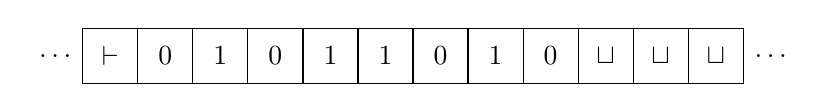
\begin{tikzpicture}
            \edef\sizetape{0.7cm}
            \tikzstyle{tmtape}=[draw,minimum size=\sizetape]
            \tikzstyle{tmhead}=[arrow box,draw,minimum size=.5cm,arrow box
            arrows={east:.25cm, west:0.25cm}]

            \begin{scope}[start chain=1 going right,node distance=-0.15mm]
                \node [on chain=1,tmtape,draw=none] {$\ldots$};
                \node [on chain=1,tmtape] {$\vdash$};
                \node [on chain=1,tmtape] {0};
                \node [on chain=1,tmtape] {1};
                \node [on chain=1,tmtape] {0};
                \node [on chain=1,tmtape] {1};
                \node [on chain=1,tmtape] {1};
                \node [on chain=1,tmtape] {0};
                \node [on chain=1,tmtape] {1};
                \node [on chain=1,tmtape] {0};
                \node [on chain=1,tmtape] {$\sqcup$};
                \node [on chain=1,tmtape] {$\sqcup$};
                \node [on chain=1,tmtape] {$\sqcup$};
                \node [on chain=1,tmtape,draw=none] {$\ldots$};
            \end{scope}
        \end{tikzpicture}
    \end{center}

    We call a set of strings Turing-recognisable \cite{Recognisable} if we can
    construct some Turing machine to recognise it, that is, every input we feed
    it that is in the language will cause the Turing machine to eventually move
    to the accept state. Notice, however, that while there are two
    ``destination'' states, $q_{\text{accept}}$ and $q_{\text{reject}}$, there
    is a third possible outcome: that our machine does not halt, but instead
    loops somewhere in its proceedings infinitely. Thus we call a set of strings
    decidable if our Turing machine always halts for its inputs, that is, for
    any input we feed it we are guaranteed to land in either $q_{\text{accept}}$
    or $q_{\text{reject}}$.

    As an example of a Turing machine in action, suppose we want to construct a
    one to accept the language $L = \{w\#w | w \in \{0,1\}\ast\}$.  This is not
    Context Free \cite{nonCFL}, meaning Turing Machines are at least more
    powerful than Push Down Automata. We construct the machine informally as
    follows:

    \begin{turing}{M}{on input $w$:}
        \item Find a decomposition of $w$ into $w_1 \# w_2$
        \item Start at the first symbol of $w_1$, replace the symbol with a
            cross, and skip forward to the first symbol of $w_2$.
            \bitem if this symbol is the same as the one you just crossed off,
            cross it off and rewind to the symbol on the right of the first
            symbol of $w_1$
            \bitem else reject
        \item Repeat this process, each time skipping forward and rewinding so
            that you are inspecting the first symbol to the right of a cross
            each time
        \item If you end up inspecting a cell with the symbol $\#$, and the
            symbols either side of it are crosses, accept
    \end{turing}

    The final thing to cover in order to understand how cellular automata such
    as the Game of Life can be used to simulate a Turing Machine is the concept
    of a Universal Turing Machine. A Universal Turing Machine is one which
    recognises the language

    $$A_{TM} = \{\braket{M,w} | M \text{ is a Turing Machine and } M
    \text{ accepts } w\} $$

    The $\braket{M,w}$ notation is used to denote the encoding of the Turing
    Machine $M$ and its input $w$ in a way that some Turing Machine would be
    able to understand and use as input. In essence, Universal Turing Machines
    are those which are capable of simulating any other Turing Machine just from
    its description and an input, and it is from this angle that we will look at
    the universality of certain cellular automata. In case this seems like a bit
    of a leap, we can simply describe the Universal Turing Machine $U$ as
    follows:

    \begin{turing}{U}{on input $\braket{M,w}$, where $M$ is a Turing Machine and
        $w$ is a string:}
        \item Run $M$ on input $w$
        \item If $M$ ever enters its accept state, accept; if $M$ ever enters
            its reject state, reject
    \end{turing}

    Note that $U$ will never halt if $M$ never halts, and so while it recognises
    the language $A_{TM}$, it does not decide it. In fact, $A_{TM}$ is called
    the Halting Problem and is undecidable: there is no way for an algorithm to
    determine whether some Turing Machine $M$ may or may not halt on input $w$,
    without simulating it itself.

    \begin{figure}
        \centering
        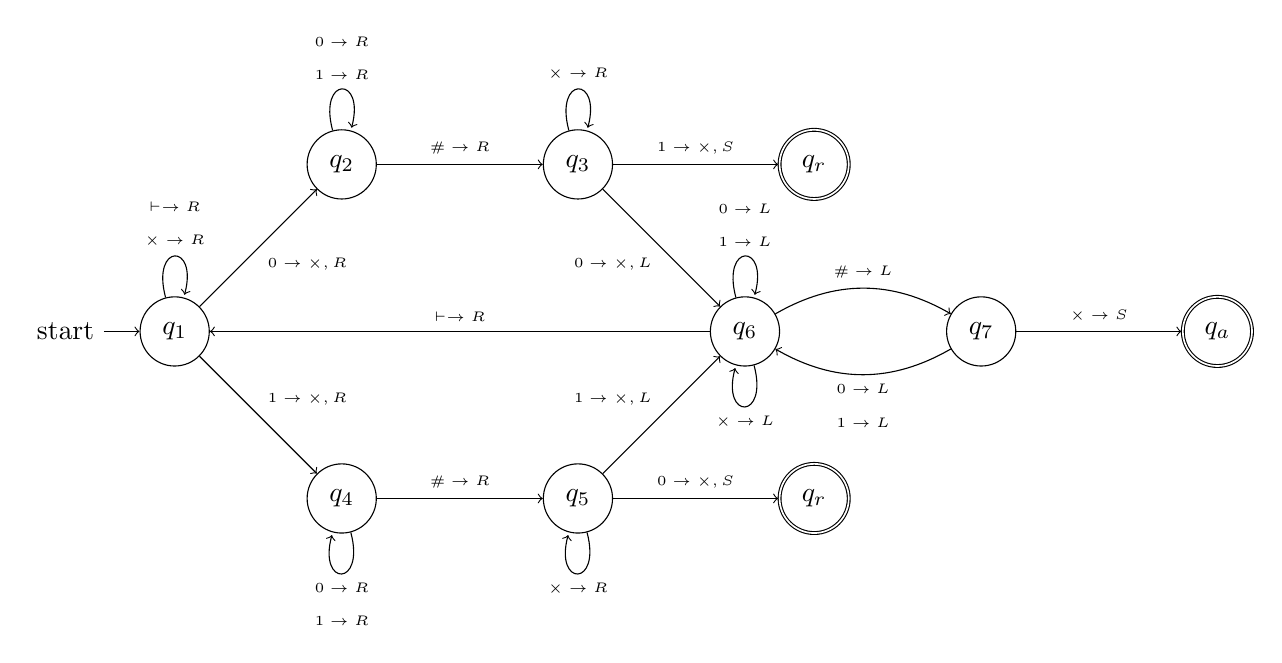
\begin{tikzpicture}[
                ->,
                node distance=3cm,
                on grid,
                auto]
            \node[state,initial]    (q1) []                     {$q_1$};
            \node[state]            (q2) [above right of=q1]    {$q_2$};
            \node[state]            (q3) [right of=q2]          {$q_3$};
            \node[state]            (q4) [below right of=q1]    {$q_4$};
            \node[state]            (q5) [right of=q4]          {$q_5$};
            \node[state]            (q6) [above right of=q5]    {$q_6$};
            \node[state]            (q7) [right of=q6]          {$q_7$};
            \node[state,accepting]  (qa) [right of=q7]          {$q_a$};
            \node[state,accepting]  (qr1) [right of=q3]         {$q_r$};
            \node[state,accepting]  (qr2) [right of=q5]         {$q_r$};

            \path[->]
            (q1)
                edge [loop above] node [align=center] {\tiny$\vdash
                    \rightarrow R$ \\ \tiny$\times \rightarrow R$} ()
                edge  node  [swap] {\tiny$0 \rightarrow \times, R$} (q2)
                edge  node  {\tiny$1 \rightarrow \times, R$} (q4)
            (q2)
                edge [loop above] node [align=center] {\tiny$0 \rightarrow R$ \\
                    \tiny$1 \rightarrow R$} ()
                edge node {\tiny$\# \rightarrow R$} (q3)
            (q3)
                edge [loop above] node {\tiny$\times \rightarrow R$} ()
                edge node [swap] {\tiny$0 \rightarrow \times, L$} (q6)
                edge node {\tiny$1 \rightarrow \times, S$} (qr1)
            (q4)
                edge [loop below] node [align=center] {\tiny$0 \rightarrow R$ \\
                    \tiny$1 \rightarrow R$} ()
                edge node {\tiny$\# \rightarrow R$} (q5)
            (q5)
                edge [loop below] node {\tiny$\times \rightarrow R$} ()
                edge node {\tiny$0 \rightarrow \times, S$} (qr2)
                edge node {\tiny$1 \rightarrow \times, L$} (q6)
            (q6)
                edge [loop above] node [align=center] {\tiny$0 \rightarrow L$ \\
                    \tiny$1 \rightarrow L$} ()
                edge [loop below] node [align=center] {\tiny$\times \rightarrow L$} ()
                edge [bend left] node {\tiny$\# \rightarrow L$} (q7)
                edge node [swap] {\tiny$\vdash \rightarrow R$} (q1)
            (q7)
                edge [bend left] node [align=center] {\tiny$0 \rightarrow L$ \\
                    \tiny$1 \rightarrow L$} (q6)
                edge node {\tiny$\times \rightarrow S$} (qa);
        \end{tikzpicture}
        \caption{A possible Turing Machine to recognise $L$}
        \label{TM:L}
    \end{figure}

    \subsection{Universality of Game of Life}
    A Turing Machine may compute a function by starting with the input to the
    function on the tape and halting with the output of the function on the
    tape. A function $f : \Sigma \ast \rightarrow \Sigma \ast$ is computable if
    some Turing Machine $M$ halts, for every input $w$, with just the result
    $f(w)$ on the tape \cite{Computable}. Thus, any model we can devise which
    could simulate the run of a Turing Machine on some input would be capable of
    computing all the functions that the Turing Machine could, and hence such a
    model would be Turing complete.

    The key to Game of Life's universal computation is its ability to create
    infinite growth, for example by using glider guns. Guns can then be
    positioned to shoot at blocks in specific locations, and doing so correctly
    can be used to move the block closer or further away. This sliding block
    memory can be used to simulate a counter \cite{Counter}. Logical AND, OR,
    and NOT gates can also be constructed using gliders, with the presence of a
    glider signifying a 1, and 0 otherwise. These three Boolean operators are
    theoretically necessary and sufficient to build a Universal Turing Machine
    \cite{BoolTM}. A fully functioning Turing Machine was designed to completion
    by Paul Rendell on 2\textsuperscript{nd} April, 2000 \cite{golTM}, which
    doubled the number on the input tape. Further extensions led to the
    development of Universal Turing Machines in February 2010 and March 2011,
    both of which were capable of simulating the Turing Machine from 2000
    \cite{golUTM1,golUTM2}.

    \begin{figure}[h]
        \includegraphics{}
        \caption{}
        \label{}
    \end{figure}

\section{More cellular automata}
    \subsection{WireWorld}
    \subsubsection{Computational Universality}
    \subsection{Rule 110}
    \subsubsection{Computational Universality}
    \subsection{Von Neumann's automaton}
    \subsection{Fractran}
    \subsection{Langton's Ant}
\section{Applications}
    \subsection{Cryptography}
\section{Firing Squad Synchronisation Problem}
\section{Majority Problem}

\bibliography{bibliography}

\end{document}
